\chapter{Product and Cost Analysis}
The Care Home is a facility that attaches great importance to safety and energy efficiency. Therefore, it is essential to check different products for certain characteristics. The following attributes are particularly important.
\begin{itemize}
	\item power consumption (sustainability)
	\item costs
	\item integration with systems
	\item compatibility
	\item maintainability
	\item lifespan
	\item customer support 
\end{itemize}

%=================================================================================
\section{Surveillance camera}
By taking the criteria into account, the closer decision was made on two models. The \textit{Bascom Pro Dom-Camera} and the \textit{Sony IP SNC-EB632R}. Dome cameras are semicircular and can be mounted on the ceiling or on a roof (as opposed to bullet cameras). Dome cameras also attract less attention. Bacom's Dome camera uses wireless data transmission and can be connected to the regular power supply. The Sony camera can be powered via Ethernet (power over ethernet) and also provides data via the same cable. Both have an IP66 standard. Thus they can be used inside as well as outside of the building. There is hardly any difference in price, which is why this does not contribute to the purchase decision. However, the wired version is more reliable as signal interference has less influence on the quality. Therefore, the first choice is the Sony camera.
\begin{figure}[h]% 
	\centering 
	\subfloat[Bascom Dome Camera]{ 
		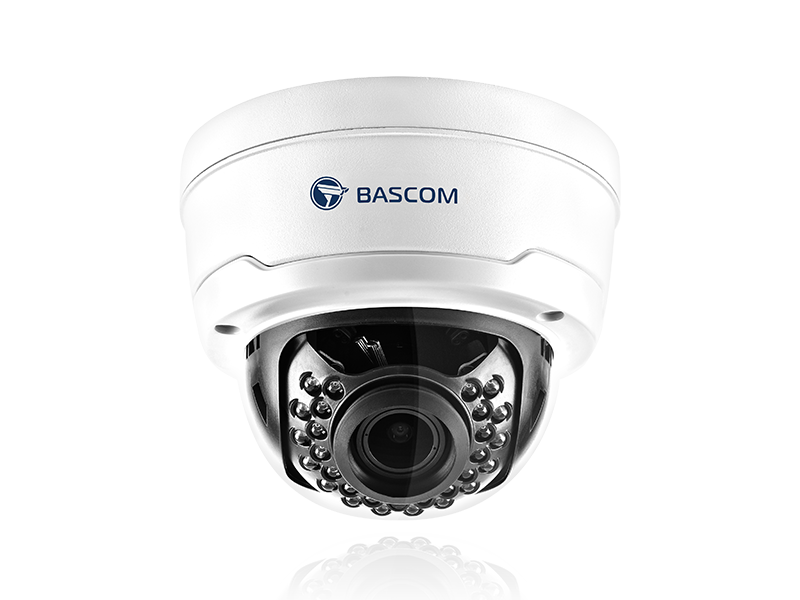
\includegraphics[width=0.4\textwidth]{images/CostAnalysis/domeCamera-pd20}% 
	} \hspace{1cm}
	\subfloat[Recorder for Dome Camera]{ 
		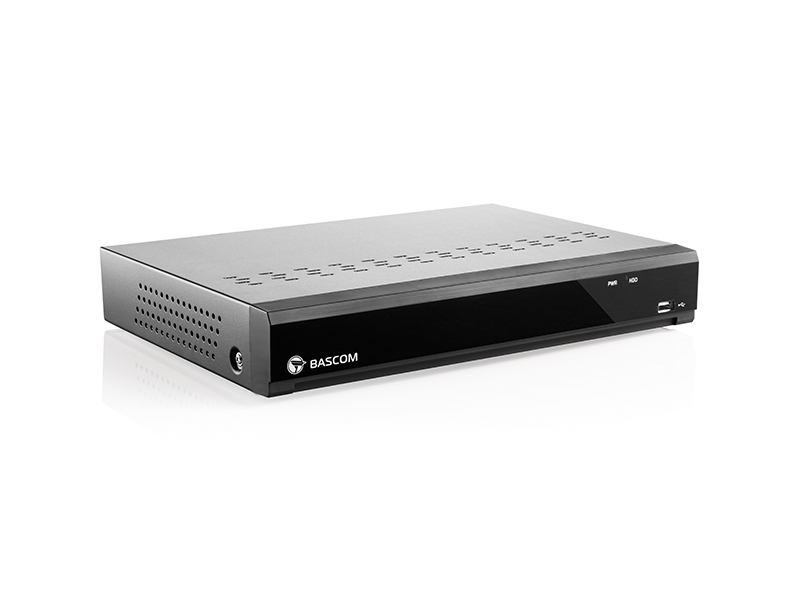
\includegraphics[width=0.4\textwidth]{images/CostAnalysis/recorder-pr4}% 
	} 
	\caption{Dome Camera System}% 
	\label{fig:domeCameraSystem}% 
\end{figure}

\begin{figure}[h]
	\centering
	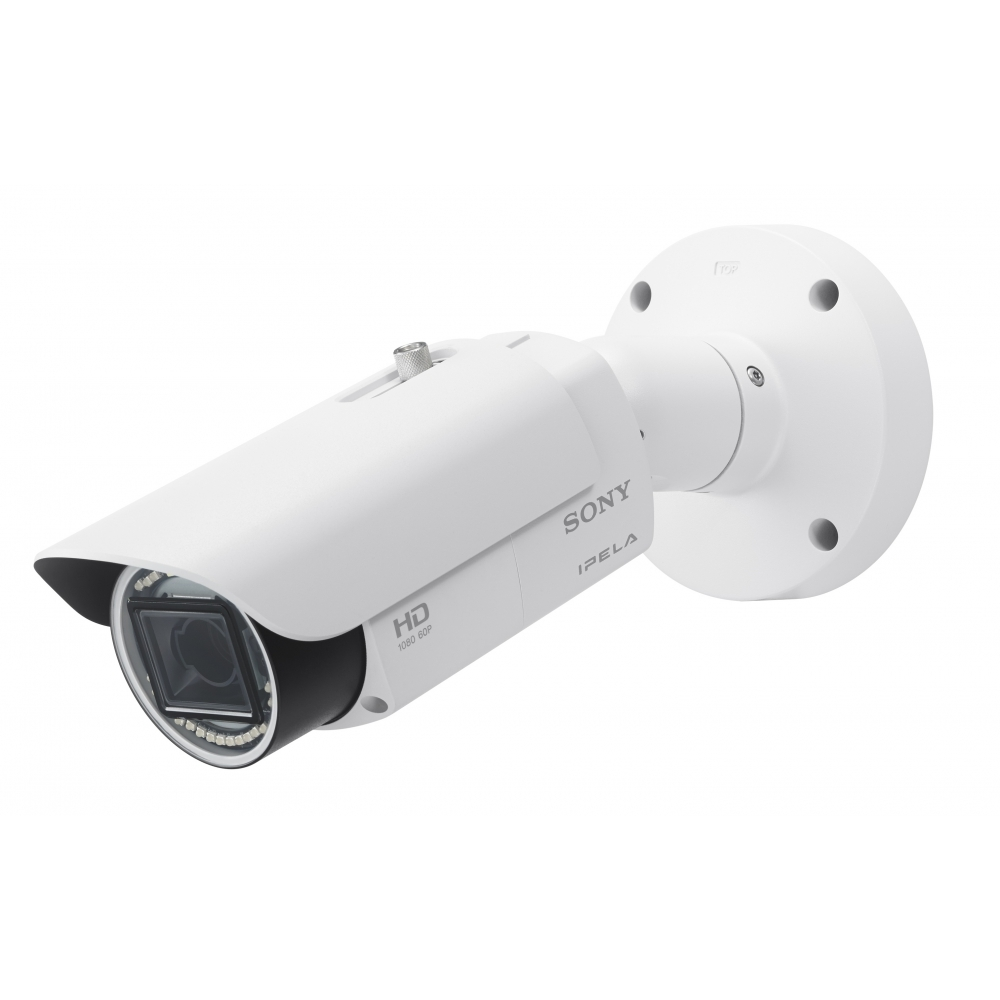
\includegraphics[width=.5\textwidth]{images/CostAnalysis/sony-ip-bullet-kamera} 
	\caption{Sony IP Bullet Camera}
	\label{fig:sonyCamera}
\end{figure}

%=================================================================================
\section{Smoke detector}
In the event of a fire, it is essential to have reliable smoke detectors in operation. Since this project aims to score points above all with customer satisfaction, inconspicuous and simple smoke detectors are preferable. There are several manufacturers that produce, for example, smart smoke detectors. Examples are Bosch, Nest or innogy. Smart devices have the advantage of being relatively easy to integrate into a system. The data can be retrieved via Wifi, Bluetooth or via web app. It is even possible to integrate the functions of the smoke detector into your own application via the API.
\\
Considering the above mentioned criteria, the choice was made for the second generation of the \textit{Nest Protect}. It scores with its simple appearance and the variety of functionality.  The price and performance of this device match very well and outperform the competition.

\begin{figure}[h]
	\centering
	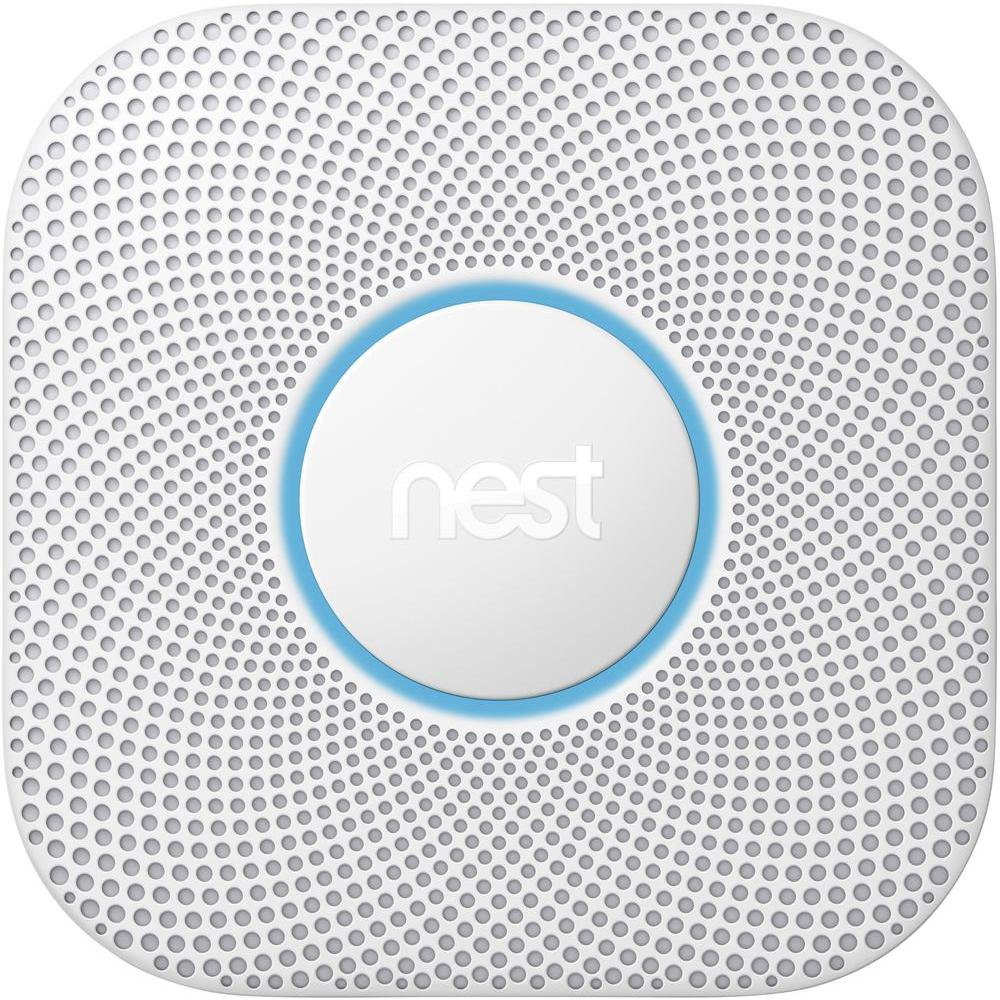
\includegraphics[width=.4\textwidth]{images/CostAnalysis/NestProtect} 
	\caption{Nest Protect Smoke Detector}
	\label{fig:smokeDetection}
\end{figure}

%=================================================================================
\section{NAS }
The network hard disk is a device that must function reliably. Important data is stored there and must be quickly accessible. That's why sufficient RAM (at least 8 GB) and a modern processor is of great importance. Another important point is of course the scalability, as well as the integration into the system, and commissioning.
\clearpage
\begin{figure}[h]
	\centering
	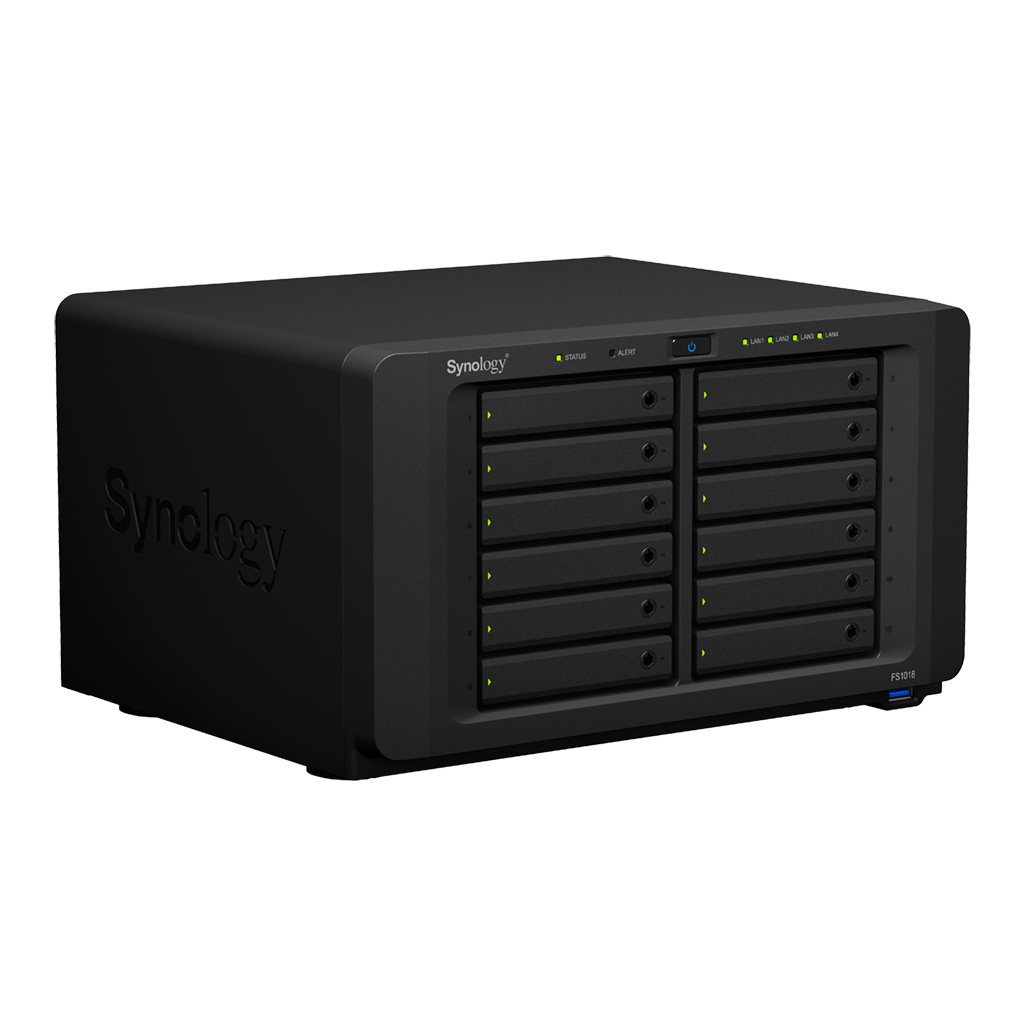
\includegraphics[width=.6\textwidth]{images/CostAnalysis/synologyFS1018} 
	\caption{NAS}
	\label{fig:nas}
\end{figure}

At this point, the \textit{Synology FlashStation FS1018} was chosen. With 12 SSD disks, it has sufficient storage capacity to store the most important data over a long period of time. The specifications are also appealing. Synology advertises their product with low latency, which is important for the application because emergency data, for example, must be retrieved quickly.

%=================================================================================
\section{Inductive and smart sensors}
In this application, inductive sensors are required to obtain the status of different furnishing objects. Examples of this are e. g. whether a door or a window is open or closed. Inductive sensors are available in different sizes, from different manufacturers. However, the choice fell on a certain sensor from Sick. The \textit{Sick IME08-1B5PSZT0S} is an inconspicuous and reliable proximity sensor that fits well into our concept. 
\newpage
\begin{figure}[h]
	\centering
	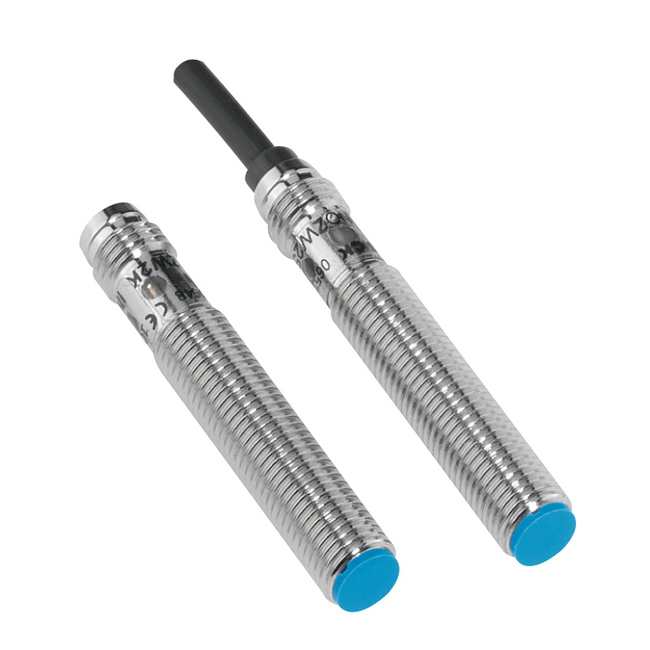
\includegraphics[width=.4\textwidth]{images/CostAnalysis/sickIni} 
	\caption{Sick inductive sensor}
	\label{fig:sickIni}
\end{figure}

Another idea is to use a smart sensor instead of an inductive sensor. The smart heating system (chapter \ref{sec:smartHeating}) enables these two systems to interact with each other in order to create an efficient cooperation. A certain smart door and window contact from Panasonic has stood out. The \textit{Panasonic KX-HNS101}.

\begin{figure}[h]
	\centering
	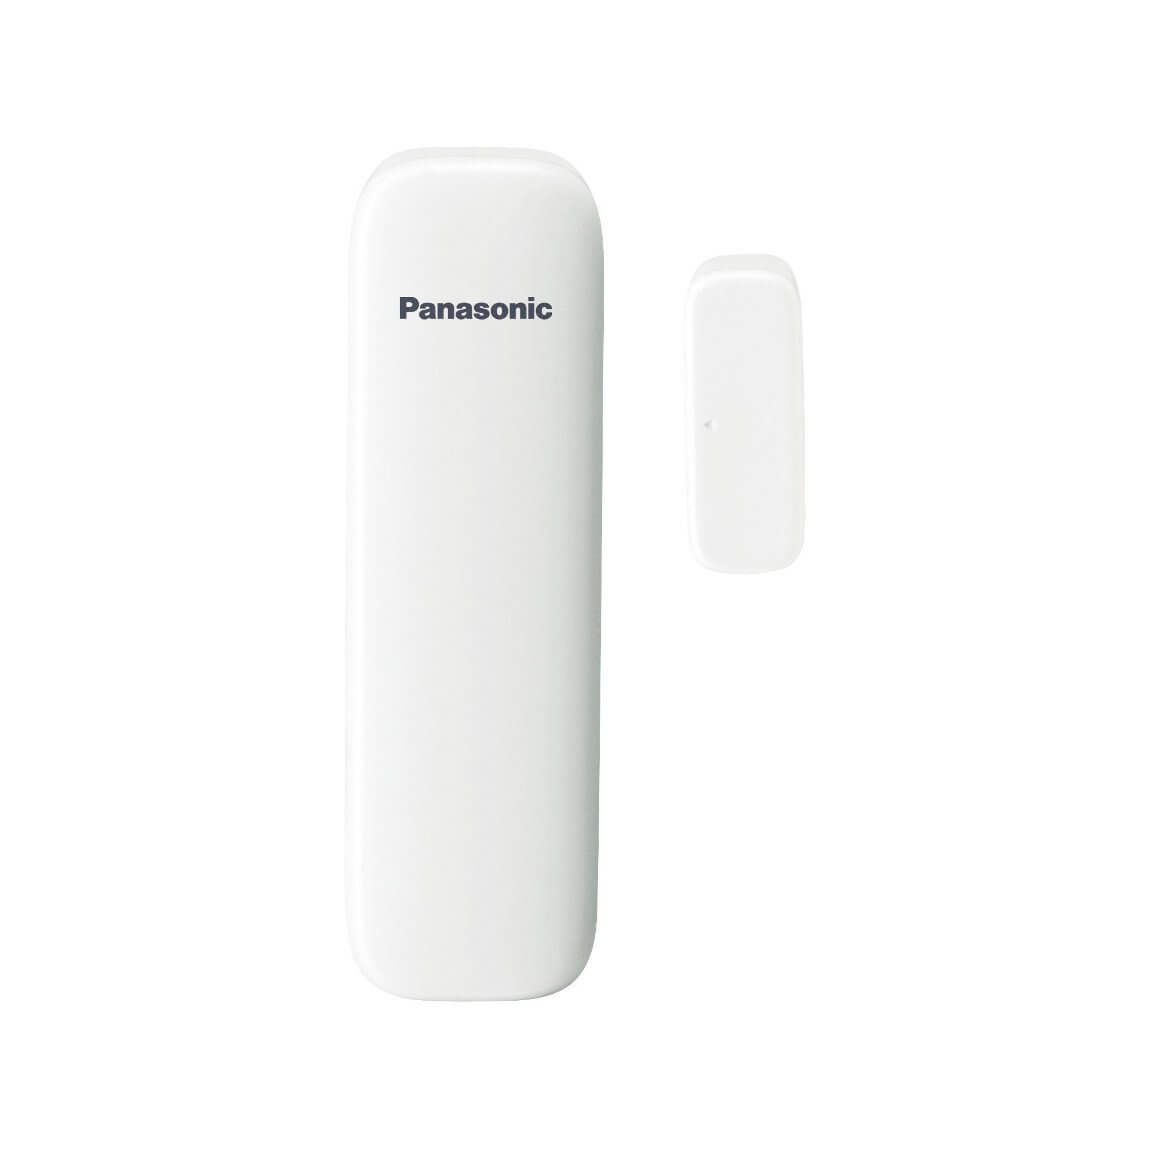
\includegraphics[width=.4\textwidth]{images/CostAnalysis/panasonicfensterkontakt} 
	\caption{Sick inductive sensor}
	\label{fig:panasonicSmart}
\end{figure}

%=================================================================================
\section{Database Server}
An important aspect of this project is the storage of data in a database. For this it is important that it is both scalable and robust. Data must be transported quickly and securely. And a lot of memory must be available. The \textit{Dell EMC PowerEdge T640} was selected for this. Because it is a tower server and not a server for the rack, the consumption is lower, which fits our needs for this project.

\begin{figure}[h]
	\centering
	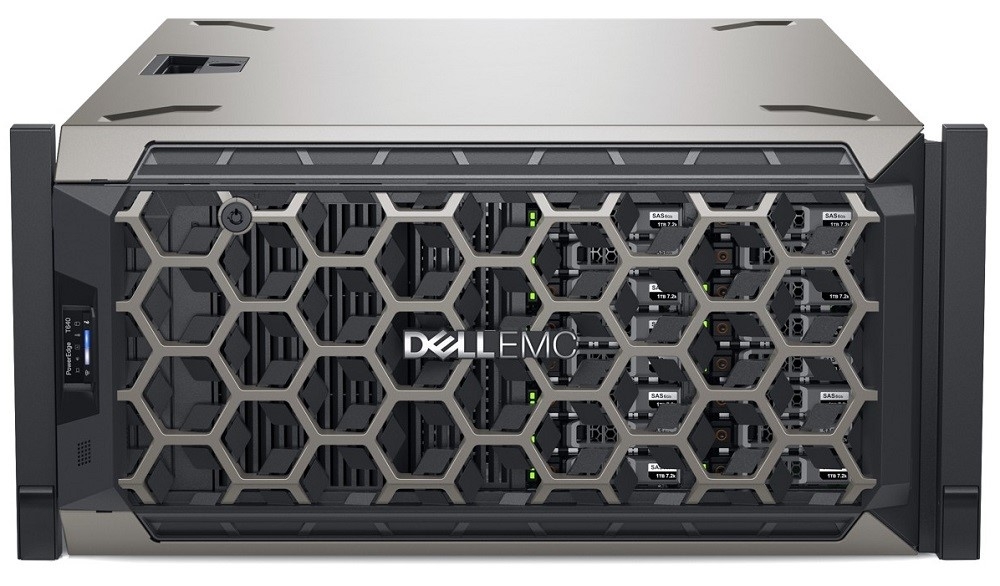
\includegraphics[width=.6\textwidth]{images/CostAnalysis/DellEMCPowerEdgeT640} 
	\caption{Dell EMC PowerEdge T640}
	\label{fig:dbServer}
\end{figure}

%=================================================================================
\section{CPU for PLC System}
PLC systems are used to process sensor data and send signals to devices. In this way, controllers can be written that receive, process sensor data and supply outputs that control actuators. This can be used to realize comfort functions. When a sensor receives a certain value, an actuator is activated which automatically opens doors or switches lights on or off, for example. Since we gained a lot of positive experience with B\&R through other projects, the choice was made for the \textit{X20CP1485 CPU}. It is characterised by its compact size, low energy consumption and extensibility. It is also capable of supporting various protocols such as POWERLINK or CAN. Thus we are flexible in development and can react dynamically to hardware changes.

\begin{figure}[h]
	\centering
	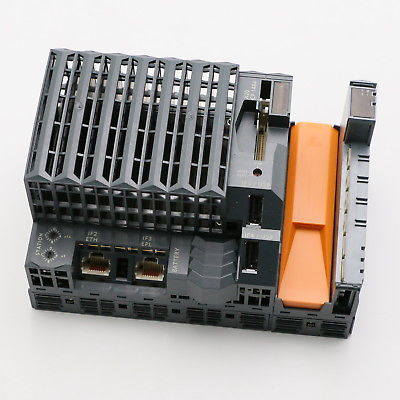
\includegraphics[width=.5\textwidth]{images/CostAnalysis/BR-Automation-X20-CP-1484} 
	\caption{B\&R CPU}
	\label{fig:brCPU}
\end{figure}

%=================================================================================
\section{Motion detectors}
Motion detectors are an important part of our application. Since mostly elderly people live in the care home, it is important that they come into contact with technical equipment as little as possible. This increases the comfort factor enormously. They do not have to deal with technical innovations, but can enjoy their stay. The motion detectors are required to control lights, for example, when a resident is in a certain area. Since we don't want the residents to feel observed, the motion detector must be very simple. It must not interfere with the environment or be technically impaired by the exterior. Since there are also many manufacturers with good equipment like Philips, Elgato or Lupusec, the choice is not easy. The price-performance ratio and simplicity are an important point. That's why we chose the \textit{Lupusec DUAL Way}.
\newpage
\begin{figure}[h]
	\centering
	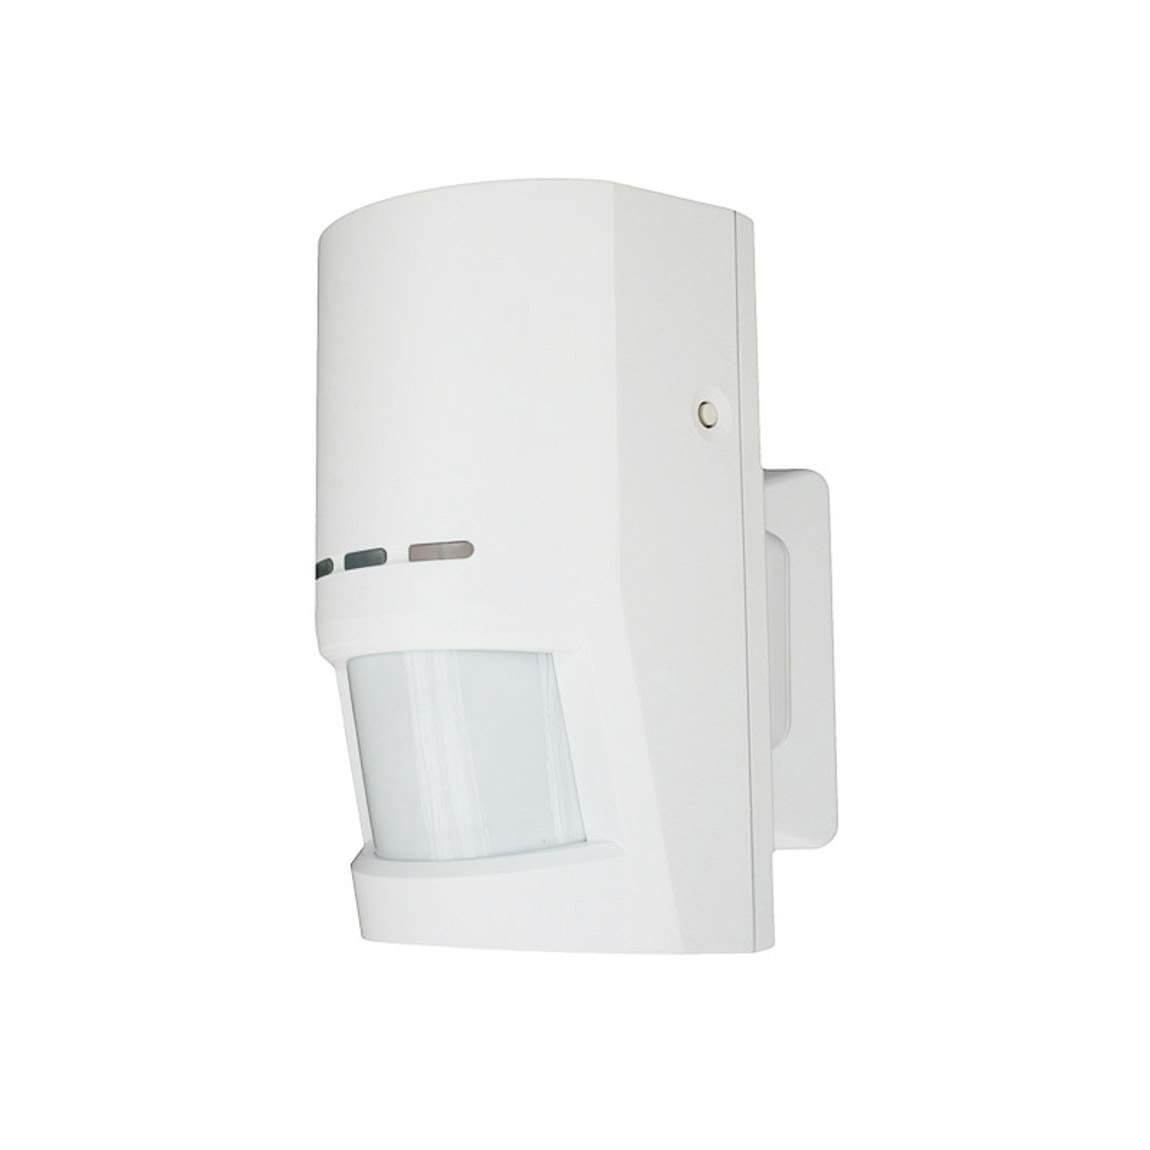
\includegraphics[width=.4\textwidth, trim=3cm 3cm 3cm 4cm, clip]{images/CostAnalysis/lupusecBewegungsmelder} 
	\caption{Lupusec DUAL Way}
	\label{fig:lupusecDual}
\end{figure}

%=================================================================================
\section{Healthcare Wristband}
A constant control of body values for patients can be very helpful to the caregivers. Classical methods such as pulse measurement or blood pressure measurement must be done manually by helpers and cost the patient time. During this time they are often not allowed to move, otherwise they can influence the values. Long-term measurements with old devices are complex and error-prone and do not give the patient a good and relaxing feeling. Our aim is to carry out long-term measurements, which the patient does not notice in the best case scenario. We use the \textit{Lenovo HW01 Smart Wristband}, which comes with a variety of features. 
\begin{itemize}
	\item pedometer
	\item sleep monitor
	\item heart rate measurement
	\item Date and time
	\item wake-up function
	\item stopwatch
	\item notifications
	\item Music playback control
	\item movement memory
	\item GPS run mode
\end{itemize}
Of course, this device does not replace special medical devices. However, it can be used for forecasting and unobtrusive monitoring, which can react quickly in an emergency.

\begin{figure}[h]
	\centering
	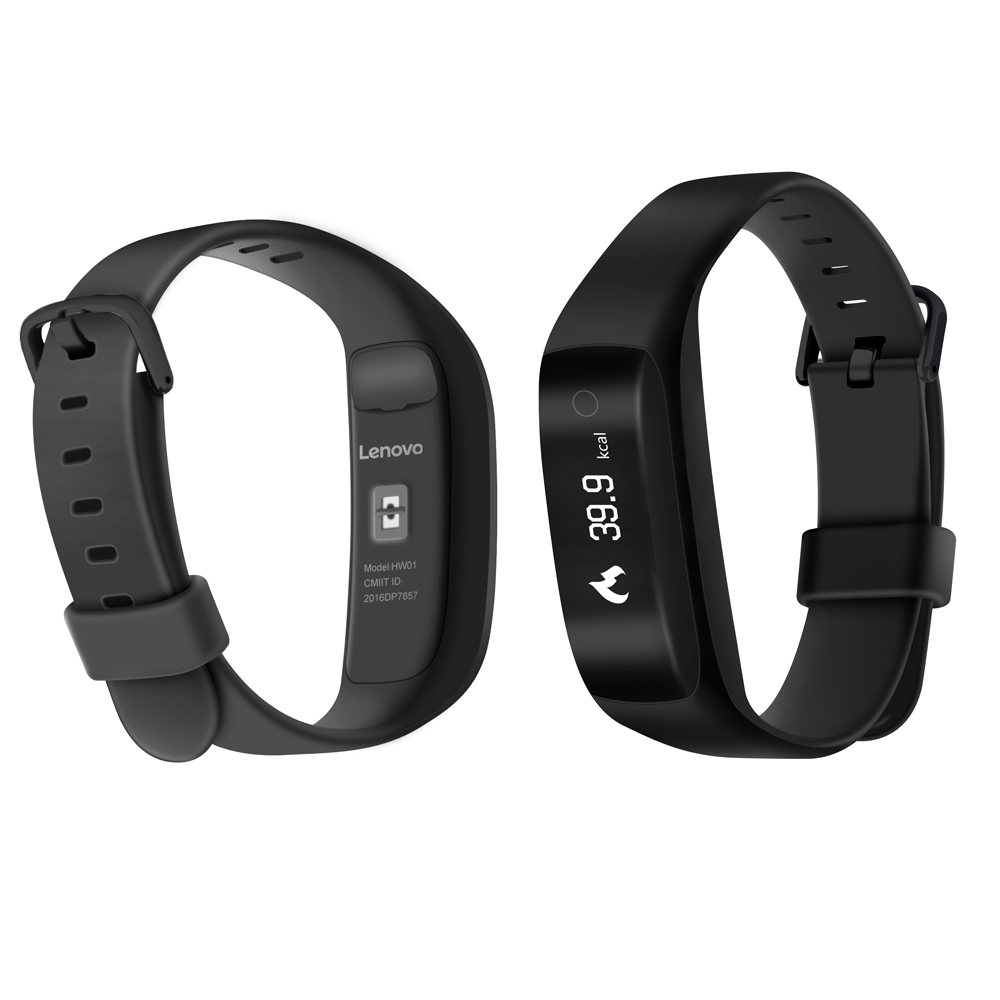
\includegraphics[width=.5\textwidth, trim=1cm 4cm 2cm 4cm, clip]{images/CostAnalysis/LenovoHW01} 
	\caption{Lenovo HW01 Smart Wristband}
	\label{fig:lenovoHealth}
\end{figure}

%=================================================================================
\section{Emergency button}
In order to offer patients the possibility to submit a message in case of emergency, we have decided to implement an emergency button. The data is then stored and evaluated centrally to prevent emergencies from being simulated or inadvertently activated. The \textit{FIBARO The Button (Z-Wave)} is a good and efficient way to realize this idea.
\newpage
\begin{figure}[h]
	\centering
	
\includegraphics[width=.4\textwidth]{images/CostAnalysis/fibaroEmergency} 
	\caption{FIBARO The Button (Z-Wave)}
	\label{fig:fibaroEmergency}
\end{figure}

%=================================================================================
\section{Smart heating system}
\label{sec:smartHeating}
A very important point in our product development is the heating of rooms. A lot of energy is lost there if the heating is not efficient. One of the market leaders in smart heating is the manufacturer Elgato. The product of our choice is the \textit{second-generation Elgato Eve Thermo}. 
\\
In addition to a simple installation, simple appearance and display, it comes with a variety of useful functions. Schedules can be set for heating schedules. It is also possible to view a consumption analysis. Both for the heating behaviour and for the energy. Another useful feature is the possibility to connect doors and window sensors with the smart heating system. As a result, the system knows when the windows and doors are opened and can regulate the heating process efficiently.
\newpage
\begin{figure}[h]
	\centering
	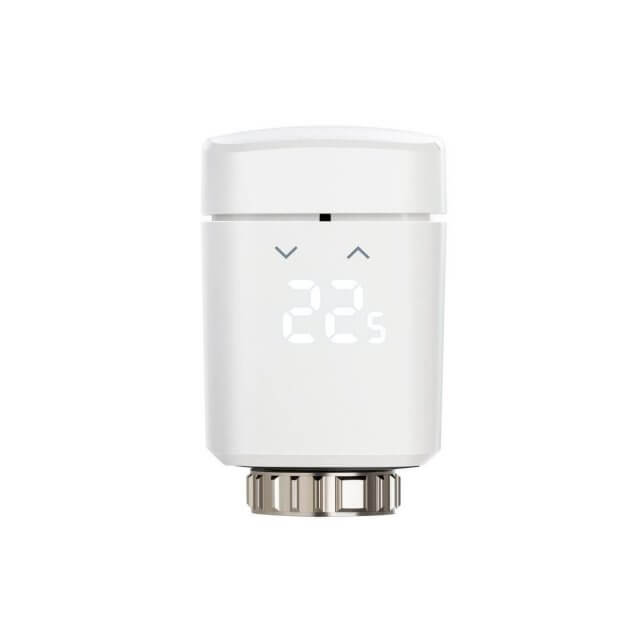
\includegraphics[width=.5\textwidth, trim=0 3cm 0 3cm, clip]{images/CostAnalysis/elgato-eve-thermo} 
	\caption{Elgato Eve Thermo}
	\label{fig:elgatoEve}
\end{figure}

%=================================================================================
\section{Water consumption}
A very important point in the care home system is the analysis and monitoring of water consumption. The data should be collected automatically and forwarded to a central point so that water consumption can be regulated. Abnormal behaviour can also be detected, for example, if someone has forgotten to turn off the water. In this case, warning signals can be sent to the staff to check that everything is in order and can act quickly in an emergency. A very interesting product is the \textit{FLUID meter}, which is used in our project.

\begin{figure}[h]
	\centering
	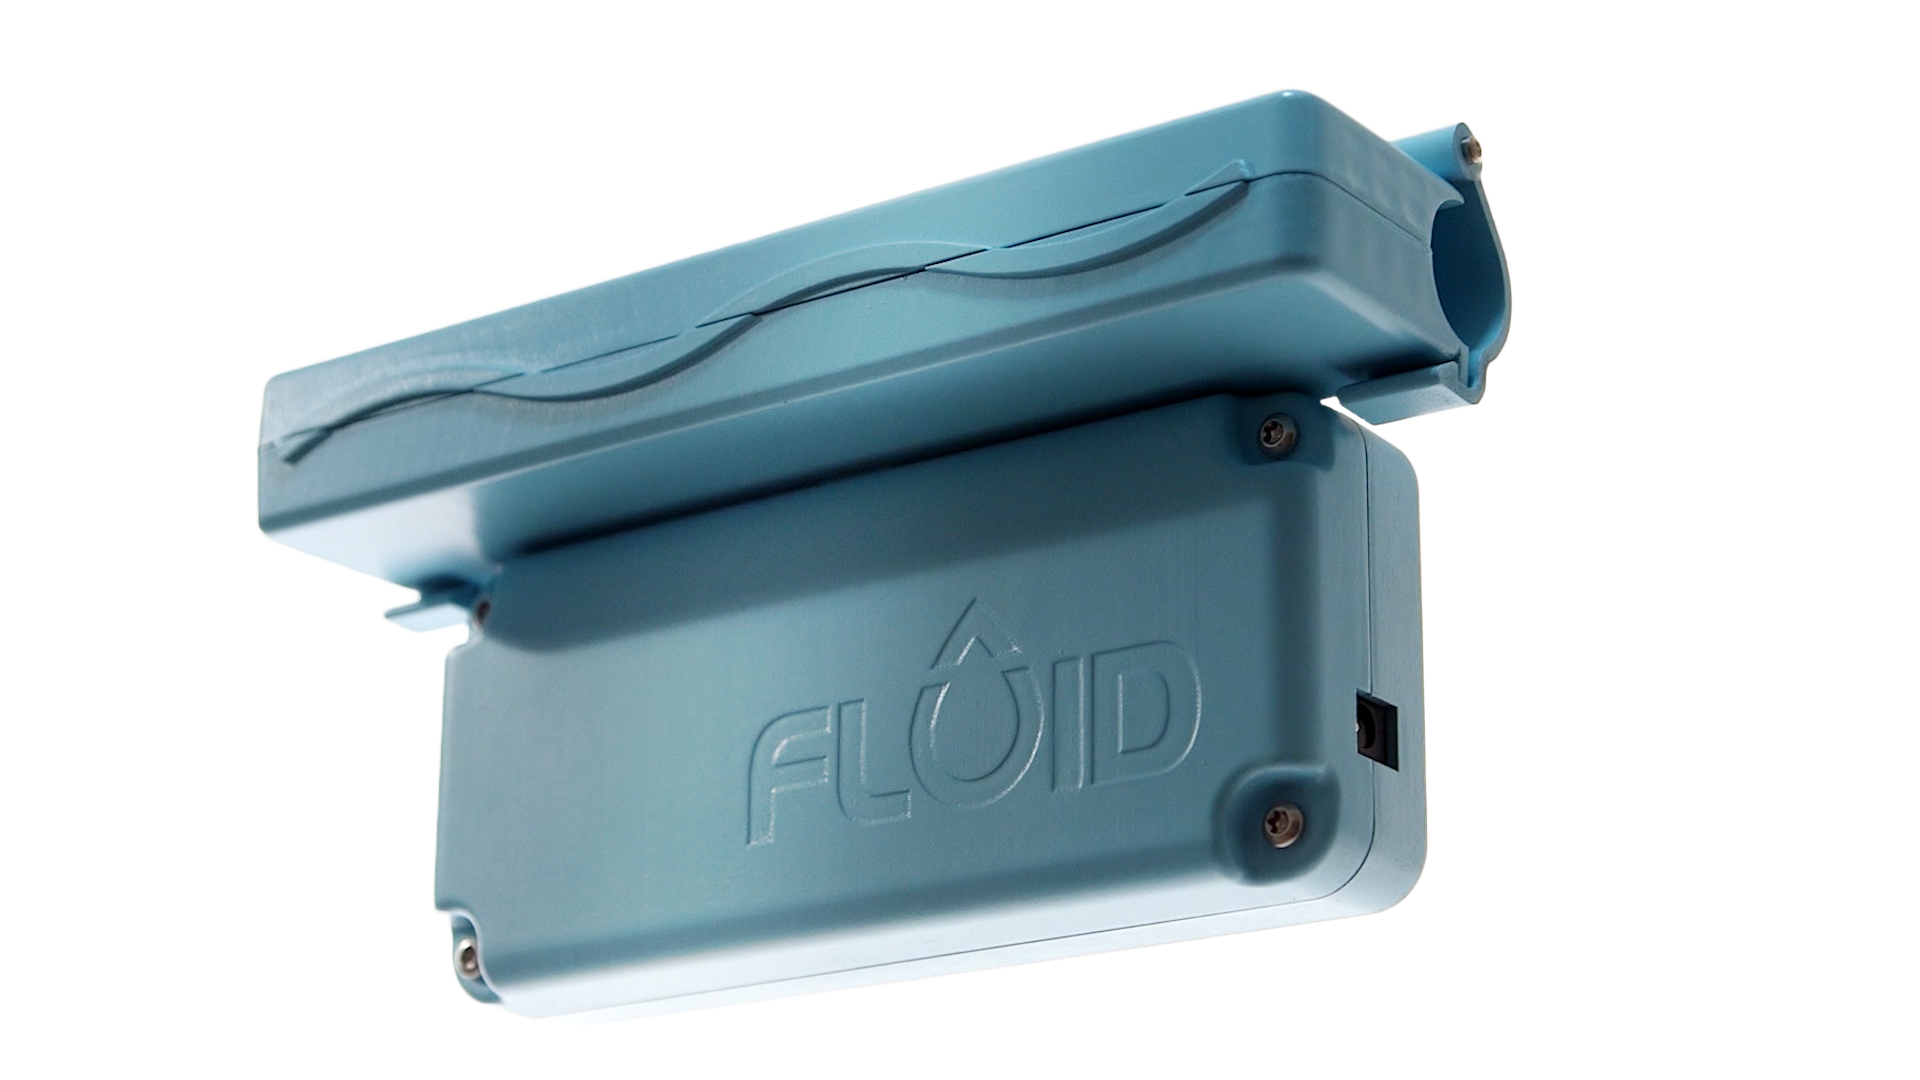
\includegraphics[width=.6\textwidth]{images/CostAnalysis/fluidMeter} 
	\caption[FLUID meter]{FLUID meter\protect\footnotemark}
	\label{fig:fluidMeter}
\end{figure}
\footnotetext{Source:\\http://www.fluidwatermeter.com/wp-content/uploads/2014/11/Fluid-Campaign.00\_00\_57\_18.Still002.png}
%=================================================================================
\section{HMI Tablets}
It makes sense to use a portable tablets to transfer information quickly to the staff. The idea is that nurses can digitally enter and retrieve patient records. With one click statistics about patients and rooms can be retrieved and managed. Another use case is that the cleaning staff has a possibility to document the cleaned rooms. Things like cleanliness or contamination can be noted. Our product of choice is the \textit{iPad Pro}, which scores points for its performance and simple appearance. Although it is more expensive than the competition, we have had good experiences with these tablets in the past, which has made our decision easier.
\\
\\
\begin{figure}[h]
	\centering
	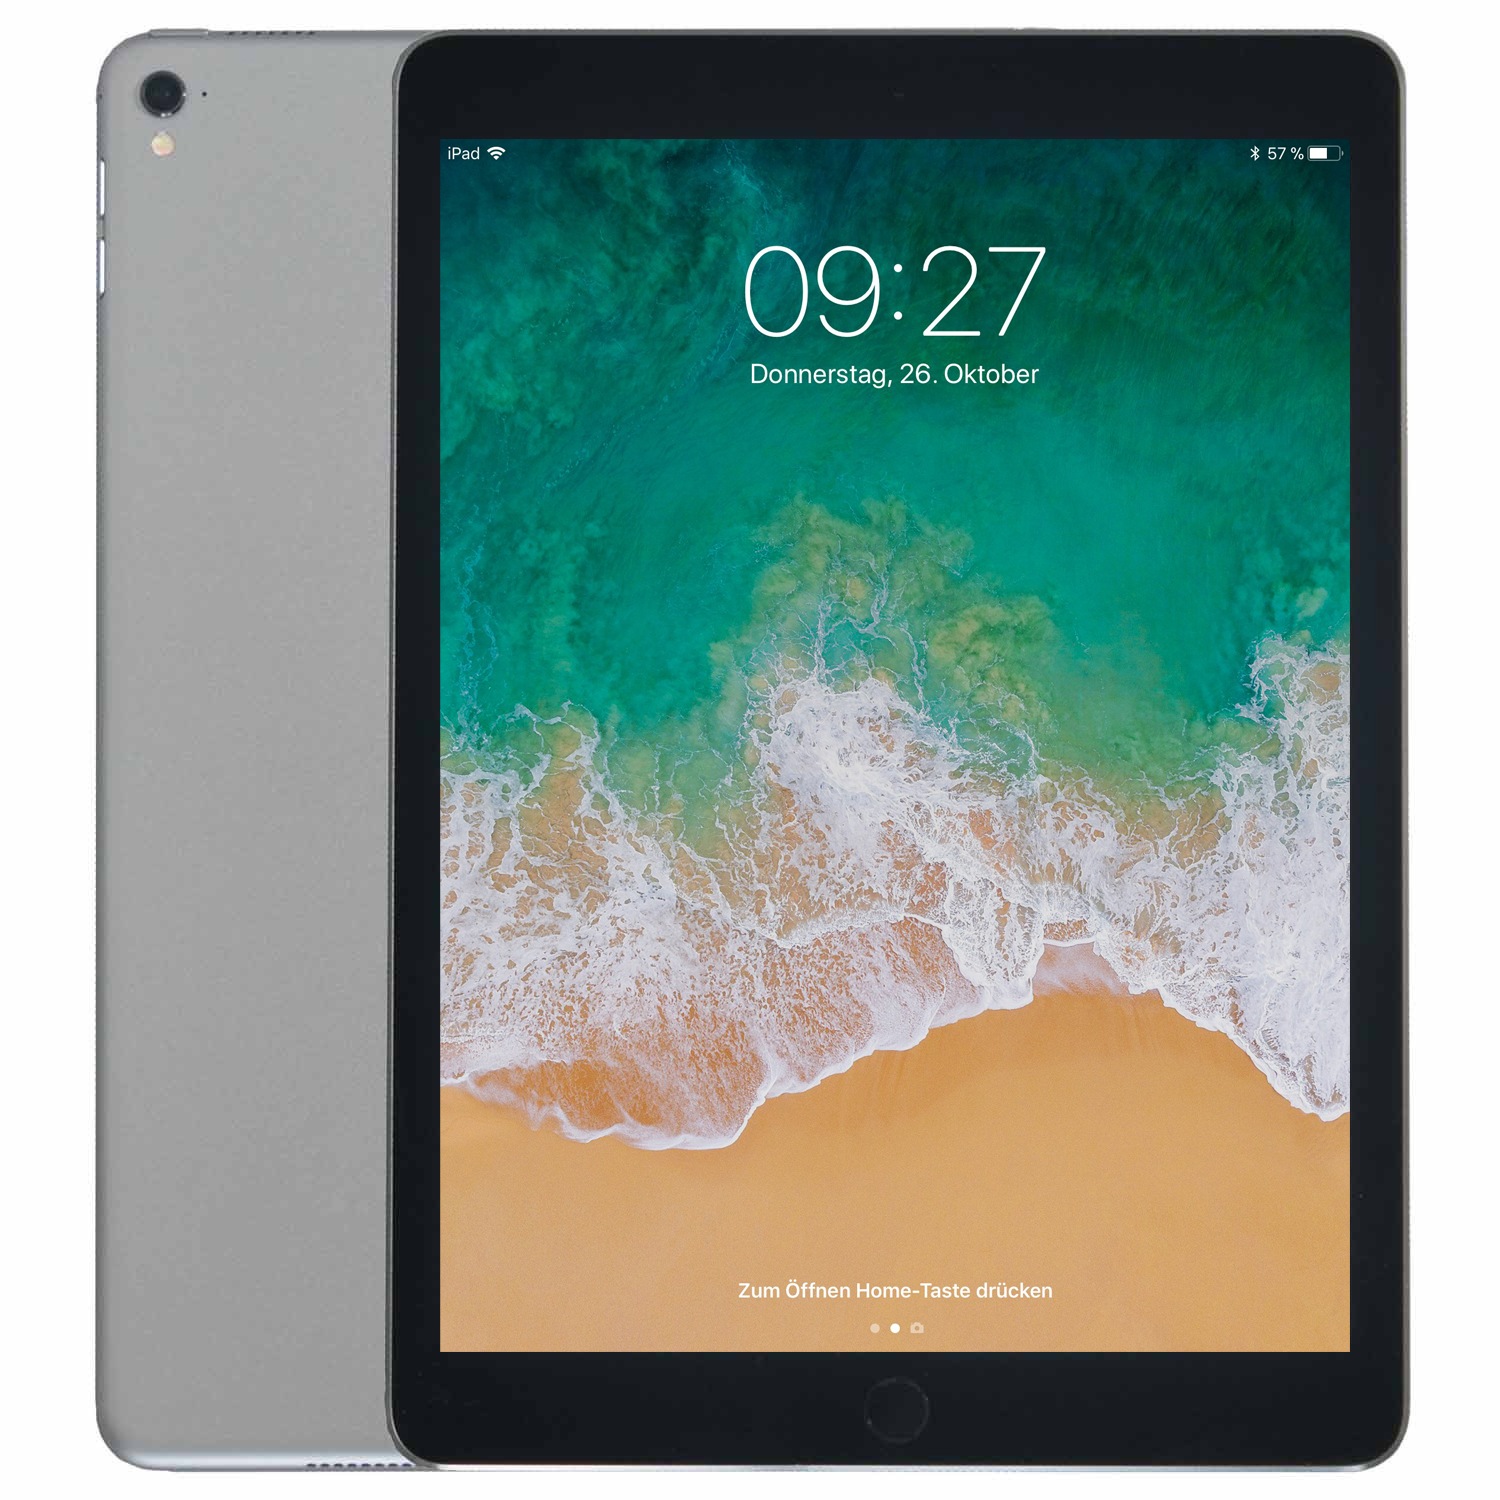
\includegraphics[width=.5\textwidth]{images/CostAnalysis/iPadPro} 
	\caption[12,9" iPad Pro]{12,9" iPad Pro\footnotemark}
	\label{fig:iPadPro}
\end{figure}
\footnotetext{Source: \\https://media.nbb-cdn.de/images/products/310000/316143/Apple\_iPadPro\_2017\_space\_Hero.jpg}
\clearpage
%=================================================================================
\section{Cost Calculation}
\begin{table}[h]
	\centering
	\renewcommand{\arraystretch}{1.9}
	\begin{tabular}{lrrr}
	Label & Price Per Unit [\officialeuro] & Amount & Cumulative Costs [\officialeuro] \\
	\hline
	Sony IP SNC-EB632R & 1,000 & 5 & 5,000\\
	Nest Protect & 130 & 120 & 15,600\\
	Synology FlashStation FS1018 & 1,600 & 2 & 3,200\\
	Panasonic KX-HNS101 & 30 & 250 & 7,500\\
	Dell EMC PowerEdge T640 & 2,000 & 2 & 4,000\\
	B\&R X20CP1485 & 2,000 & 2 & 4,000\\
	Lupusec DUAL Way & 200 & 160 & 32,000\\
	Lenovo HW01 Smart Wristband & 30 & 120 & 3,600\\
	FIBARO The Button (Z-Wave) & 50 & 110 & 5,500\\
	Elgato Eve Thermo 2. Gen & 80 & 110 & 8,800\\
	FLUID meter & 250 & 130 & 32,500\\
	12,9" iPad Pro & 1,000 & 20 & 20,000\\
	\hline
	%Products Total & & & \textbf{xxx}\\
	Working Hours (most likely)& 1172 & 100 & 117,200 \\
	Overhead Costs &  &  & 40,000\\
	\hline
	\hline
	Nett Total & & & 293,905\\
	+ VAT 20\% & & & 58,781\\
	\hline
	\hline
	\textbf{Total} & & & \textbf{352,686}
	\end{tabular}
\end{table}
